\title{Mayfly -- Rapid, Accessible, Reproducible Research}
\author{Nelson Auner and Cody Buntain \\ nelson@nelsonauner.com  and cbuntain@cs.umd.edu}
\date{\today}

%\documentclass[10pt,twocolumn]{article}
\documentclass[10pt,a4]{article}

\usepackage{courier}       %for coding - nelson
\usepackage{lscape}	% For landscape views
\usepackage{fullpage}	% Give me 1in margins all around
\usepackage{graphicx}	% For including pictures
\usepackage[colorlinks=true,linkcolor=blue]{hyperref}	% For hyper links
\usepackage{parskip}	% No paragraph indention
\usepackage[small,compact]{titlesec}	% Less spacing between titles
\usepackage{listings}	% For including code
\usepackage{sgame}	% For typesetting games
\usepackage{amsmath}	% for plain text in math mode
\usepackage{algpseudocode}	% For pseudocode typesetting
\usepackage[margin=1in]{geometry}

\def\thesection{\arabic{section}} 
\def\thesubsection{\alph{subsection}} 
\def\thesubsubsection{\roman{subsubsection}} 

\begin{document}

\maketitle

\section{Introduction}
% Discuss the value of reproducible research and easy file access
In the midst of the current data explosion and the subsequent complexity of analysis pipelines, it is becoming increasingly difficult to reproduce scientific results in a manual fashion.
These issues cumulate into a significant barrier to verification and validation, leading to a growth in publication and wide-spread acceptance of erroneous results with limited recourse for correction. 
The Open Science Data Cloud (OSDC) has significant potential to alleviate these issues with consistent and shared access to duplicate data stores, but it currently lacks straightforward methods for online publication or facilitating access to research results.
Fortunately, as data science becomes more main stream, and barrier to entry comes down, many solutions for facilitating analytics like IPython's Notebook and R-Studio are now available. 
Additionally, the significant adoption of mobile devices has lead to a plethora of solutions for file sharing across multiple systems: Dropbox, Google Drive, Microsoft's Azure, and Apple's iCloud are all examples of such solutions.
Integrating these analytics and storage solutions with the OSDC has real power to capitalize on the  both platforms in a way that could cause real impact in the scientific community and lead to a better quality of research across the field.
To that end, this project aimed to integrate Dropbox's sharing capabilities, tools for research presentation in Python and R, and the OSDC platform to support rapid, accessible, and reproducible research.

\section{Technical Details}
% Dropbox, IPython, and R-studio

We achieved this project's goals by creating a small suite of tools for publishing research code and results online and for quickly installing and configuring existing software analytic packages.
As mentioned, several popular programming languages for data analysis now have such analytic platforms specifically for supporting rapid and demonstrable code.
Of particular interest here are IPython's Notebook environment and R's Knitr package, which enable simple authoring of HTML-based web reports for code and results. 
Our suite of tools automatically installs these environments as well as Dropbox's client on OSDC virtual machines in a nearly hands-free manner.
After performing any sort of analysis in either IPython or R, the researcher can then leverage our Dropbox-based publication tool to convert their analysis workflows and results to simple HTML pages and automatically publish them directly through Dropbox's public folder API.
The researcher is then given a URL, such as \url{https://dl.dropboxusercontent.com/u/66442241/kdd.html}, she can then share with colleagues for review.


\section{Data Visualization}
In addition to easily creating and sharing reproducible research, Mayfly encourages large and interactive visualizations. In traditional reports, visualizations are constrained to the size of an email attachment or journal page, and are almost always static (non-interactive). 
Mayfly, however, puts all visualizations on the users dropbox, enabling large and more complex visualizations to be easily shared. In addition, Dropbox now supports client-side javascript, so visualizations written in \texttt{D3} or with google charts can be viewed interactively by not only the code author, but any colleagues as well. 

%figures - put in?

\section{Example Workflow}

With the software installed using the Mayfly tools, one can use either IPython's notebook or R for data analysis with relative ease.
For IPython, one need only start the notebook, begin one's work, save the notebook, and call \texttt{dropboxPublisher} on the resulting file, which automatically publishes the HTML version of the file to Dropbox for others to see (refer to Figure \ref{fig:ipythonProc}).

\begin{figure}[htbp]
\begin{center}
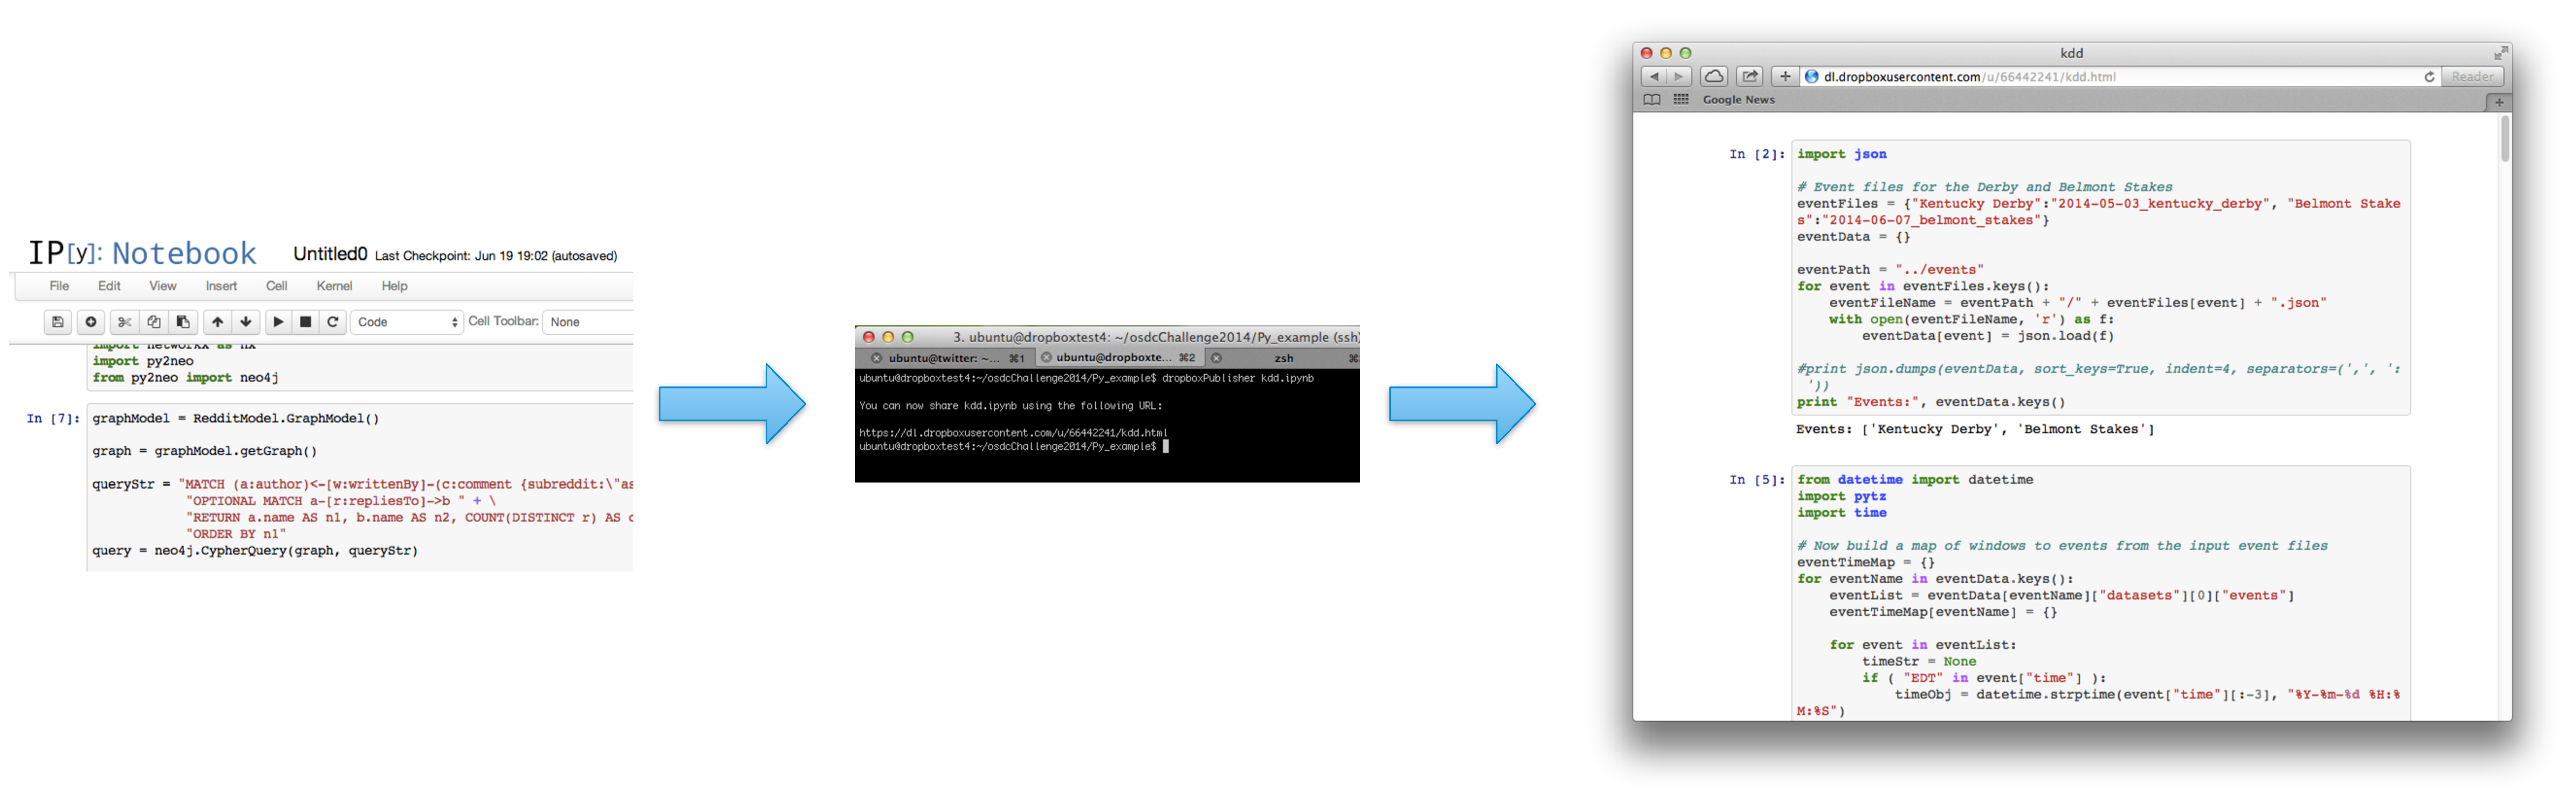
\includegraphics[width=0.9\textwidth]{flow.pdf}
\caption{IPython Notebook Process}
\label{fig:ipythonProc}
\end{center}
\end{figure}

In addition, we briefly describe a sample workflow with R, investigating the characteristics of three types of iris flowers. Mary, the researcher already has an algorithm that she wants to use, but needs to use high-powered computing. She also wants to create visualizations to help explain her results to her coauthors, without having to FTP images back and forth from her remote computer. She has used linux but is not a computer expert.

First, she runs the \texttt{setup} command to install the necessary programs, without having to understand \texttt{apt-get}, dependencies, or other problems. She then follows the instructions to link her dropbox account, and then simply runs her script with the preface \texttt{mayfly IrisAnalysis.R}  The program returns the dropbox url where she can view the report, and easily share with coworkers. In addition, her visualizations are embedded in the report, including interactive visualizations, so that her non-statistical coworkers can understand her analysis better. These advances allow Mary to quickly spot errors in her script, share her results with colleagues, and explain her analysis clearly to even remote viewers. 

\section{Conclusion}

In brief, empowering OSDC users with the tools to conduct, share, and review research in a rapid and reproducible way should be a high priority for the organization in order to gain adoption and generate higher impact in the field.
The Mayfly toolkit provides a small step in that direction with its collection of tools to facilitate rapid research that can be easily published to the public for review, reproduction, and verification.

\appendix
\section{Code Location}

\begin{description}
\item[OSDC Snapshot] To facilitate rapid adoption of the Mayfly toolkit, we have construct a beta snapshot instance that can be made public and pushed out to any OSDC user.
\item[Github Repository] To allow existing OSDC users (and any researcher in general) to make use of this rapid, reproducible research framework, we have also made our source code public at a Github Repository at the following location: \url{https://github.com/cbuntain/osdcChallenge2014}
\end{description}

\end{document}